\documentclass[11pt,a4paper]{article}

\PassOptionsToPackage{numbers,compress}{natbib}
\usepackage[margin=25mm]{geometry}
\usepackage[numbers,sort&compress]{natbib}
\usepackage{lmodern}
\setlength{\emergencystretch}{2em}

\usepackage[utf8]{inputenc}
\usepackage[T1]{fontenc}
\usepackage{hyperref}
\usepackage{url}
\usepackage{microtype}
\usepackage{amsmath,amssymb,amsfonts,mathtools}
\usepackage{booktabs}
\usepackage{tabularx}
\usepackage{graphicx}
\graphicspath{{figures/}}
\setkeys{Gin}{draft=false}
\usepackage{xcolor}
\usepackage{nicefrac}
\usepackage{tikz}
\usetikzlibrary{arrows.meta,positioning,fit,calc,matrix}

\newcommand{\method}{\textsc{CoGround-VLM}}
\newcommand{\R}{\mathbb{R}}
\newcommand{\KL}{\mathrm{KL}}
\newcommand{\Diag}{\mathrm{Diag}}
\newcommand{\BCE}{\mathrm{BCE}}
\newcommand{\softmax}{\mathrm{softmax}}
\newcolumntype{Y}{>{\raggedright\arraybackslash}X}
\newcolumntype{L}[1]{>{\raggedright\arraybackslash}p{#1}}
\newcommand{\TBD}{\textsc{tbd}}
\newtheorem{proposition}{Proposition}
\newtheorem{theorem}{Theorem}

\title{\method: Differentiable Patch-Token Co-Clustering for Visual Grounding in Vision-Language Models}
\author{Herv\'e Trinh\\Independent Researcher\\
\href{mailto:trinh.herve@gmail.com}{\texttt{trinh.herve@gmail.com}}}
\date{}
\hypersetup{pdftitle={CoGround-VLM: Differentiable Patch-Token Co-Clustering for Visual Grounding in Vision-Language Models},pdfauthor={Hervé Trinh},colorlinks=true,linkcolor=blue!45!black,citecolor=blue!45!black,urlcolor=blue!45!black}
\begin{document}

\maketitle

\begin{abstract}
Vision-language models can generate fluent descriptions without consistently exposing the local visual evidence behind their words. This paper proposes \method, a differentiable patch-token co-clustering module with simplex-constrained assignments $U,V$ and a compact block interaction matrix $B$. The structured state supports alignment losses, support diagnostics, and a route to generation control. The formulation distinguishes the general soft-assignment least-squares block solution from occupancy averaging, which is exact for hard assignments, and establishes conditional reconstruction and supported-mass properties. The historical experimental summaries report support AUROC $0.713$--$0.928$ across a 480-run synthetic study and an increase from $0.631$ to $0.981$ in a 160-run cluster-count study. On frozen Gemma 4 E2B with a custom RefCOCO split, the earlier five-seed layer-zero head reaches pointing accuracy $0.215\pm0.031$ versus $0.138$ for untrained cosine, while spatial AUROC remains near chance. These comparisons do not isolate a co-clustering advantage from learned capacity, and the earlier decoding-combo configuration did not enable a generation intervention. The original experimental summaries are retained as exploratory observations; the code supplies corrected learned controls and an effective vocabulary-logit prior. Those corrected experiments have not been executed for this version; generation faithfulness and broader transfer remain open empirical questions.
\end{abstract}

\section{Introduction}
\label{sec:intro}

Large vision-language models (VLMs) produce fluent answers and captions, yet they still generate unsupported objects, attributes, and relations when linguistic priors dominate local visual evidence \cite{rohrbach2018object,li2023pope}. A central problem is that local alignment stays implicit: the model has cross-attention, but it does not keep a compact record of which patches support which tokens.

This work treats local grounding as a structured latent object instead of leaving it as a side effect of attention. The proposed \method\ module converts local affinities into latent blocks through differentiable patch-token co-clustering. These blocks regularize alignment, produce interpretable evidence maps, and bias decoding toward visually supported content. The intended interface reuses a co-clustered patch-token state across training losses, diagnostics, and generation; its empirical value must be tested against learned alternatives.

The analysis also specifies the role of the bottleneck. With fixed assignments, the latent block matrix solves a least-squares reconstruction problem; in the ideal block-constant case, it recovers the true affinities exactly; and under an explicit ordering assumption, the decoding bias shifts more attention mass toward supported patches. These are modest results, but they make the role of the bottleneck and the decoding prior easier to read.

The claim is narrow: stronger grounding is \emph{not} assumed to solve hallucination in general. The investigation focuses on settings where outputs depend on verifiable local evidence. Controlled synthetic studies complement the real-data evaluation with known patch-token support structure, allowing direct measurement of support discrimination, decoding-mass shifts, and misspecification robustness. The same structure also acts as a probe of where visual information remains accessible inside a frozen decoder stack, and the reported results indicate that this is most useful at the earliest LM tap.

The paper makes five contributions:
\begin{itemize}
    \item a differentiable co-clustering formulation for patch-token alignment in VLMs, together with token-level support scores that expose reusable grounding structure;
    \item mechanism-level guarantees for least-squares optimality, exact recovery in the ideal block-constant regime, and supported-mass monotonicity under the decoding bias;
    \item historical summaries of a 480-run synthetic comparison against an unconstrained low-rank control across a $32\times$ noise range;
    \item a historical 160-run cluster-count study describing behavior within the matched block-generator family;
    \item an exploratory RefCOCO layer scan and five-seed early-feature probe, together with an explicit account of its learned-baseline and decoding limitations.
\end{itemize}

\section{Related Work}
\label{sec:related}

\paragraph{Grounded vision-language modeling.}
Grounded multimodal systems expose links between image regions and text, either through explicit region tokens or through cross-attentional fusion \cite{li2023blip2,microsoft2023kosmos2,liu2024llava}. They make local evidence accessible, but usually do not compress it into a stable structure reusable across decoding steps.

\paragraph{Hallucination and faithfulness.}
Object hallucination has been studied in captioning and multimodal instruction following through diagnostics such as CHAIR and POPE \cite{rohrbach2018object,li2023pope}. This version does not benchmark such full hallucination suites; instead, it focuses on the lower-level grounding signal that later mitigation systems could exploit. The proposed approach makes grounding an explicit latent structure between representation learning and decoding, complementing these hallucination diagnostics.

\paragraph{Adjacent mitigation baselines and novelty boundary.}
Recent hallucination-mitigation methods intervene at decoding time or inside attention, for example through visual contrastive decoding, rollback-style penalties, or selective reweighting of informed visual tokens \cite{leng2024vcd,huang2024opera,arif2025paint}. Semantically grounded supervision methods such as SeGroS provide a stronger training-time comparison point \cite{kim2026segros}. The contribution examined here is a co-clustered patch-token state shared by alignment regularization, support diagnostics, and generation-time control.

\paragraph{Co-clustering and latent block models.}
Co-clustering jointly partitions the two axes of a matrix into interpretable homogeneous blocks \cite{dhillon2003itcc,govaert2013coclustering}. The formulation follows the latent-block perspective in which row and column assignments summarize structure rather than only pairwise similarity \cite{govaert2013coclustering,govaert2008bernoulli,nadif2010continuous,govaert2018mutual}. It also connects to low-rank tri-factorization, where the block matrix becomes a learned intermediate object rather than a post-hoc visualization \cite{ding2006onmtf}.

\section{Method}
\label{sec:method}

\subsection{Patch-token affinity and latent blocks}

Given an image-prompt pair, let $P \in \R^{N_p \times d}$ denote visual patch embeddings and $T \in \R^{N_t \times d}$ text-token embeddings at a chosen fusion layer. The affinity matrix is defined as
\[
S \in \R^{N_p \times N_t}, \qquad S = PWT^{\top}/\sqrt{d},
\]
where $W \in \R^{d \times d}$ is learnable. In practice, $S$ can also be initialized from aggregated cross-attention maps; the bilinear form is simply the cleanest default parameterization.

Two learned soft assignment matrices describe the memberships,
\[
U \in \Delta^{N_p \times K_p}, \qquad V \in \Delta^{N_t \times K_t},
\]
with row-wise simplex constraints. $U$ assigns each patch to a mixture of visual blocks and $V$ assigns each token to a mixture of textual blocks. The historical implementation used the occupancy-normalized block average
\[
B_{\mathrm{occ}} = D_u^{-1}U^{\top}SV D_v^{-1},
\qquad
D_u = \Diag(U^{\top}\mathbf{1}), \quad D_v = \Diag(V^{\top}\mathbf{1}),
\]
where the diagonal matrices contain cluster occupancies. This is exact least squares for hard assignments, not general soft memberships. The current default instead uses
\[
B=(U^\top U)^+U^\top SV(V^\top V)^+,
\]
with a configurable numerical pseudoinverse threshold. The reconstructed affinity matrix is
\[
\hat{S} = UBV^{\top}.
\]

The assignments are parameterized by lightweight MLP heads followed by row-wise softmax,
\[
U = \softmax(f_p(P)), \qquad V = \softmax(f_t(T)).
\]
The reference configuration uses $K_p=K_t=16$, which keeps the block space compact while leaving enough capacity for object- and phrase-level structure.

\paragraph{Least-squares interpretation of the block matrix.}
The block matrix also admits a simple formal interpretation when the assignments are fixed.
\begin{proposition}
\label{prop:ls-block}
Assume $U \in \R^{N_p \times K_p}$ and $V \in \R^{N_t \times K_t}$ have full column rank. The minimizer of
\[
\min_{B \in \R^{K_p \times K_t}} \|S - U B V^{\top}\|_F^2
\]
is
\[
B^{\star} = (U^{\top}U)^{-1}U^{\top}SV(V^{\top}V)^{-1}.
\]
More generally, if the Gram matrices are rank-deficient, the Moore-Penrose pseudoinverse yields the minimum-norm solution. In the hard-assignment regime, $U^{\top}U = D_u$ and $V^{\top}V = D_v$, so the historical occupancy-normalized block average recovers the exact least-squares optimum.
\end{proposition}
\paragraph{Proof sketch.}
Differentiating the Frobenius objective with respect to $B$ and setting the result to zero gives the normal equations
\[
U^{\top}U\,B\,V^{\top}V = U^{\top}SV.
\]
Solving them yields the stated expression whenever the Gram matrices are invertible; the pseudoinverse handles the degenerate case. The hard-assignment claim follows because one-hot memberships make the Gram matrices diagonal cluster-count matrices. This observation does not by itself prove better grounding, but it shows that the block matrix is a principled summary of $S$ rather than an arbitrary extra head.

\paragraph{Compression and exact-recovery regime.}
\begin{proposition}
\label{prop:rank-recovery}
For any $U \in \R^{N_p \times K_p}$, $V \in \R^{N_t \times K_t}$, and $B \in \R^{K_p \times K_t}$, the reconstruction $\hat{S} = UBV^{\top}$ obeys
\[
\operatorname{rank}(\hat{S}) \le \min\{\operatorname{rank}(U),\operatorname{rank}(B),\operatorname{rank}(V)\} \le \min\{K_p,K_t\}.
\]
If $U$ and $V$ encode hard assignments with nonempty clusters and the ground-truth affinity matrix $S$ is block-constant with respect to those assignments, then the occupancy-normalized estimator $B = D_u^{-1}U^{\top}SV D_v^{-1}$ reconstructs $S$ exactly.
\end{proposition}
\paragraph{Proof sketch.}
The rank bound is immediate from the product structure of $\hat{S}$. For the exact-recovery claim, each pair $(i,j)$ belongs to a unique block $(a,b)$, so $(UBV^{\top})_{ij}=B_{ab}$. When $S$ is block-constant, every within-block average equals the true block value, which is exactly what the occupancy-normalized estimator computes. Thus the reconstructed matrix matches $S$ entrywise. This proposition clarifies why the bottleneck can simultaneously compress the affinity map and remain lossless in the ideal block-structured regime.

\subsection{Training objective}

The co-clustering loss is
\[
\mathcal{L}_{\mathrm{cc}} = \operatorname{MSE}(\hat S,\mathrm{stopgrad}(S)) + \lambda_{\mathrm{ent}}\big(H(U)+H(V)\big)
+ \lambda_{\mathrm{bal}}\big(\KL(\bar U\,\|\,u_0)+\KL(\bar V\,\|\,v_0)\big),
\]
where $H(\cdot)$ is row-wise entropy, $\bar U$ and $\bar V$ are empirical cluster occupancies, and $u_0,v_0$ are target priors, typically uniform. The entropy term discourages overly diffuse assignments; the balancing term discourages occupancy collapse without ruling it out mathematically. The corrected main configuration includes true grounding supervision. Stopping gradients through the reconstruction target alone does not remove self-reference, because $\hat S$ still depends on $S$ through $B$.

When grounding annotations are available, a binary or soft target matrix $G$ defines the additional grounding loss
\[
\mathcal{L}_{\mathrm{ground}} = \BCE\big(\sigma(\hat{S}), G\big).
\]
The full training objective is
\[
\mathcal{L} = \mathcal{L}_{\mathrm{task}} + \lambda_{\mathrm{cc}}\mathcal{L}_{\mathrm{cc}} + \lambda_{\mathrm{ground}}\mathcal{L}_{\mathrm{ground}},
\]
where $\mathcal{L}_{\mathrm{task}}$ is the base VLM loss. If dense alignment labels are unavailable, the same formulation can use phrase-grounding supervision or pseudo-labels from an external grounding system.

\subsection{Block-aware decoding}

The original theoretical proposal reuses latent blocks through an attention bias. It is retained here as a conditional mechanism, not a claim about an installed attention hook. Let $A_{ij}$ denote the attention logit from token position $j$ to patch $i$ inside the decoder. The proposed modified logit is
\[
A'_{ij} = A_{ij} + \lambda_{\mathrm{dec}}\,\mathrm{stopgrad}\big((UM_jV^{\top})_{ij}\big),
\]
where $M_j = g(h_j) \in \R^{K_p \times K_t}$ is a token-conditioned block matrix predicted from the current decoder state $h_j$. In effect, the decoder is encouraged to concentrate on a small subset of coherent patch-token blocks instead of repeatedly rediscovering local evidence from scratch.

The generic adapter does not install this attention intervention. Its effective implementation is instead a static vocabulary-logit prior. From the final prompt hidden state $h$, a network predicts $M(h)$. Candidate vocabulary embeddings have textual assignments $C_{w\ell}$, and scores
\[
a_\ell=\max_i(UM(h))_{i\ell},\qquad r_w=\sum_\ell a_\ell C_{w\ell}
\]
are normalized and added to actual generation logits through a logits processor, optionally restricted to plausible base-model candidates. This prompt-conditioned bias is reused at every decoding step; it is not recomputed from generated hidden states. An independent-assignment control uses its own patch and candidate-token heads. Contextual training tokens and vocabulary embeddings differ, so effective generation guidance must be measured rather than inferred from an auxiliary grounding loss.

\paragraph{Supported-set mass increases with the decoding bias.}
\begin{proposition}
\label{prop:mass-shift}
Fix a decoding step $j$ and define
\[
q_i(\lambda) = \frac{\exp(a_i + \lambda c_i)}{\sum_{\ell=1}^{N_p}\exp(a_{\ell}+\lambda c_{\ell})},
\qquad
c_i = (UM_jV^\top)_{ij},
\]
where $a_i$ are the base patch logits. For any subset $G \subseteq \{1,\dots,N_p\}$, let $Q_G(\lambda)=\sum_{i\in G} q_i(\lambda)$. If $c_i \ge c_{i'}$ for all $i \in G$ and $i' \notin G$, then $Q_G(\lambda)$ is nondecreasing in $\lambda$. The increase is strict whenever the inequality is strict on a set carrying nonzero probability mass.
\end{proposition}
\paragraph{Proof sketch.}
Differentiate the softmax expectation to obtain
\[
\frac{d}{d\lambda} Q_G(\lambda) = \operatorname{Cov}_{q(\lambda)}(\mathbf{1}_G, c).
\]
Under the assumed ordering, patches in $G$ always receive support scores at least as large as patches outside $G$, so the covariance is nonnegative. Hence increasing $\lambda_{\mathrm{dec}}$ cannot reduce the total attention mass assigned to the supported set in this simplified regime. The ordering assumption is not established by the proposition. This result concerns the proposed fixed-logit intervention; it does not prove that the implemented vocabulary prior changes patch attention or reduces hallucination.

\paragraph{What the theory does and does not claim.} These results are best read as sanity checks, not as a proof that co-clustering solves hallucination in general. They establish narrower properties of the mechanism: optimal block reconstruction, exact recovery in the ideal block-structured regime, monotone supported-mass shift, and monotone descent for the isolated co-clustering subproblem. Appendix~\ref{app:theory} provides complete proofs.

\subsection{Interpretability signal and complexity}

For the proposed attention mechanism at a token position $t$, let $M_t$ denote the token-conditioned block matrix used when scoring that decoding step. The support score is defined as
\[
r(t) = \max_i (UM_tV^{\top})_{i,t},
\]
which can be used to flag tokens that lack credible visual support. The same block structure also yields reordered heatmaps and block trajectories across decoding steps.

Dense affinity construction costs $\mathcal{O}(N_pN_td)$ after the patch projection, whose dense bilinear cost is $\mathcal{O}(N_pd^2)$. The compact latent state has $N_pK_p+N_tK_t+K_pK_t$ entries, but constructing and reconstructing dense affinities still incurs patch-token matrix costs. The Gram solve adds terms $\mathcal{O}(N_pK_p^2+N_tK_t^2+K_p^3+K_t^3)$. Compact state does not make dense reconstruction linear in the cluster counts alone.

\begin{figure}[t]
\centering
\resizebox{\linewidth}{!}{%
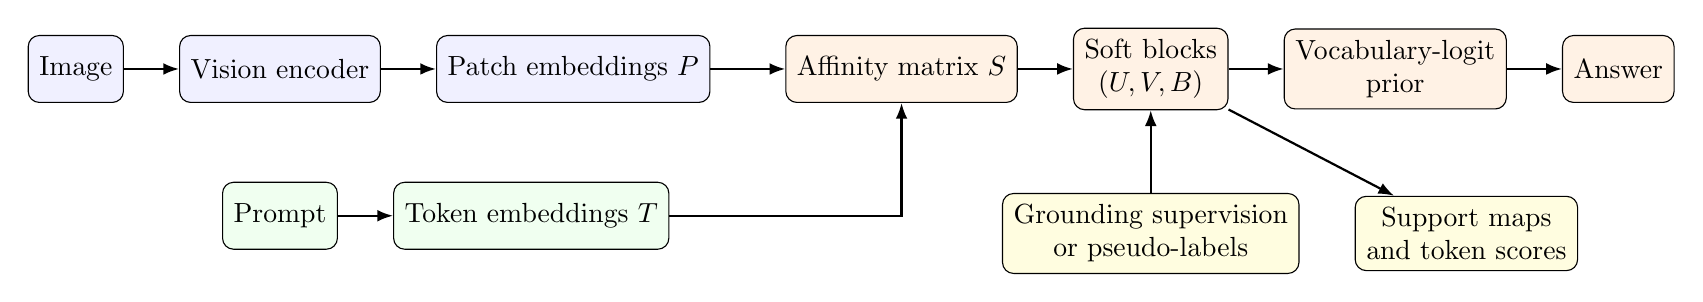
\begin{tikzpicture}[
  node distance=0.75cm and 0.7cm,
  box/.style={draw,rounded corners,align=center,minimum height=0.85cm,inner sep=4pt},
  arr/.style={-{Latex[length=2mm]},thick}
]
\node[box, fill=blue!6] (img) {Image};
\node[box, fill=blue!6, right=of img] (vision) {Vision encoder};
\node[box, fill=blue!6, right=of vision] (patch) {Patch embeddings $P$};

\node[box, fill=green!6, below=1.0cm of vision] (prompt) {Prompt};
\node[box, fill=green!6, right=of prompt] (text) {Token embeddings $T$};

\node[box, fill=orange!10, right=0.95cm of patch] (aff) {Affinity matrix $S$};
\node[box, fill=orange!10, right=of aff] (blocks) {Soft blocks\\$(U,V,B)$};
\node[box, fill=orange!10, right=of blocks] (decode) {Vocabulary-logit\\prior};
\node[box, fill=orange!10, right=of decode] (answer) {Answer};

\node[box, fill=yellow!12, below=1.05cm of blocks] (ground) {Grounding supervision\\or pseudo-labels};
\node[box, fill=yellow!12, right=of ground] (maps) {Support maps\\and token scores};

\draw[arr] (img) -- (vision);
\draw[arr] (vision) -- (patch);
\draw[arr] (patch) -- (aff);
\draw[arr] (prompt) -- (text);
\draw[arr] (text.east) -| (aff.south);
\draw[arr] (aff) -- (blocks);
\draw[arr] (blocks) -- (decode);
\draw[arr] (decode) -- (answer);
\draw[arr] (ground) -- (blocks);
\draw[arr] (blocks) -- (maps);
\end{tikzpicture}%
}
\caption{Overview of \method. Patch-token interactions form latent blocks for supervision and support maps. The implemented generation branch adds a vocabulary-logit prior; the attention-bias formula is a separate theoretical proposal.}
\label{fig:pipeline}
\end{figure}

\section{Experimental Setup}
\paragraph{Evidence status.}
This section describes the historical setup retained from the original manuscript. Figure-level summaries and sanitized RefCOCO aggregates are bundled to reproduce its numerical illustrations. Raw synthetic runs, dataset manifests, full prediction logs, and trained checkpoints are not present, so the reported campaign and significance tests cannot be independently reconstructed from this release. The corrected code changes the soft solver, spatial conventions, and controls; its prospective protocol is described separately below.
\label{sec:setup}

\subsection{Backbone and common environment}

All reported real-data runs use a single open-weight backbone, \texttt{google/gemma-4-E2B-it}, under its original Apache~2.0 release terms. This paper remains deliberately narrow: it asks whether the co-clustering bottleneck provides a statistically reliable grounding mechanism and a useful probe of where visual structure survives inside one modern decoder-only VLM. Unless explicitly stated otherwise, the Gemma 4 backbone is frozen and only the co-clustering head is trained; the earlier decoding-combo label did not in fact enable the decoding module.

The earlier manuscript records the following environment. Jobs ran in bf16 with PyTorch 2.9.1+cu128 on two NVIDIA A100 80GB PCIe GPUs; the reported experiments were executed in parallel across the two devices, while each individual training or evaluation run still occupies one GPU at a time. The host provides 128 CPU cores and 251~GB RAM. The text hidden size is 1536, the vision tower produces 768-dimensional features that are projected to 1536 through \texttt{embed\_vision}, and the visual sequence contains 260 tokens (a $16\times16$ spatial grid plus four special tokens). Unless noted otherwise, the RefCOCO runs use batch size 1, gradient accumulation 8, AdamW, weight decay 0.01, max gradient norm 1.0, mixed precision bf16, and the historical target builder. These hardware and layout details are reported provenance, not a newly verified integration result.

The historical study reports four scopes on top of this shared setup: \textbf{S$_{\mathrm{massive}}$}, a 480-run synthetic comparison across 20 seeds, six noise levels, and four methods; \textbf{K$_{\mathrm{mis}}$}, a 160-run synthetic study of cluster-count misspecification with $K_{\mathrm{true}}=8$ and $K_{\mathrm{pred}}\in\{2,4,6,8,12,16,24,32\}$; \textbf{L$_{\mathrm{scan}}$}, a single-seed RefCOCO scan over 10 tap layers together with matched cosine baselines; and \textbf{L$_{\mathrm{seed}}$}, a five-seed RefCOCO study at layer $0$ with the head-only configuration plus grounding-loss and decoding-prior combos.

\subsection{Data, prompts, and metrics}

The main grounded dataset is RefCOCO \cite{yu2016refcoco}, which is built on COCO images \cite{lin2014coco}. The training split contains 6000 image-expression pairs drawn from val1, val2, val3, testA, and testB. The validation split contains 500 pairs from val0 and is held fixed throughout the study. Boxes are stored as normalized $[x_1,y_1,x_2,y_2] \in [0,1]^4$ coordinates. Every example uses the same prompt: ``Carefully observe the region circled in the image. Describe it in one short noun phrase.'' The token span target is fixed to $[[0,32]]$. The paper focuses on support-map quality on the 500-example val0 split rather than on noun-phrase exact match.

These are custom historical partitions, not a verified official RefCOCO test protocol. Without the original manifests, split isolation and image disjointness cannot be audited. The historical study evaluates the token-conditioned support maps directly using pointing accuracy, Recall@5 / @10, and AUROC for separating patches inside versus outside the reference box. The main real-data baseline is a same-layer cosine affinity with no trained head. The primary synthetic metrics are support AUROC and supported-mass shift, together with reconstruction and cluster-recovery diagnostics when relevant. The five-seed layer-$0$ summary reports mean $\pm$ standard deviation and paired two-sided $t$-tests against the cosine baseline or between matched variants.

\begin{table}[htbp]
\caption{Reported experiments on Gemma 4 E2B.}
\label{tab:data}
\centering
\footnotesize
\setlength{\tabcolsep}{3pt}
\setlength{\tabcolsep}{4pt}
\begin{tabularx}{\linewidth}{@{}L{.12\linewidth}L{.13\linewidth}L{.20\linewidth}Y Y@{}}
\toprule
Scope & Data & Size & Purpose & Main measurements \\
\midrule
$\textbf{S}_{\mathrm{massive}}$ & Synthetic block recovery & $20$ seeds $\times$ $6$ noises $\times$ $4$ methods & Test whether CoGround beats an unconstrained low-rank factorization across a wide noise range & Support AUROC, supported-mass shift, paired $t$-tests \\
$\textbf{K}_{\mathrm{mis}}$ & Synthetic block recovery & $10$ seeds $\times$ $8$ $K_{\mathrm{pred}}$ values $\times$ $2$ methods & Test robustness when the predicted cluster count differs from the true count & Support AUROC, supported-mass shift \\
$\textbf{L}_{\mathrm{scan}}$ & RefCOCO val0 & $10$ taps $\times$ $1$ seed + $10$ cosine baselines & Identify where the trained head beats same-layer cosine similarity & Pointing accuracy and gap versus cosine \\
$\textbf{L}_{\mathrm{seed}}$ & RefCOCO val0 & $5$ seeds $\times$ $3$ training conditions at layer $0$ & Test reproducibility and objective interaction at the best tap & Pointing, Recall@5 / @10, AUROC, paired $t$-tests \\
\bottomrule
\end{tabularx}
\end{table}

The reported experiments still do \emph{not} include multi-backbone transfer, RefCOCOg, POPE, CHAIR, HallusionBench, Winoground, SugarCrepe, or ARO. Those broader evaluations remain future work once aligned fine-tuning and additional backbones are in place.

\subsection{Assets and licenses}
\label{sec:assets}

Asset provenance forms part of the experimental specification. RefCOCO examples inherit the original COCO image restrictions rather than a single dataset-wide license, so the source images are not redistributed with the paper materials. Likewise, the Gemma 4 E2B weights remain governed by the original Apache~2.0 model license. Synthetic data are generated on the fly from the reported seeds and hyperparameters.

\begin{table}[htbp]
\caption{Frozen assets and provenance information for the reported experiments.}
\label{tab:assets}
\centering
\footnotesize
\setlength{\tabcolsep}{3pt}
\setlength{\tabcolsep}{4pt}
\begin{tabularx}{\linewidth}{@{}L{.16\linewidth}L{.23\linewidth}Y Y@{}}
\toprule
Asset family & Frozen identifier & Role & Terms / provenance notes \\
\midrule
Gemma 4 E2B backbone & Released Gemma 4 E2B weights & Frozen backbone for all reported RefCOCO runs & Apache~2.0 \\
RefCOCO training split & $6000$ pairs from val1 / val2 / val3 / testA / testB & Training data for layer scans and multi-seed runs & RefCOCO annotations on COCO images; inherits source-image restrictions \\
RefCOCO validation split & $500$ pairs from val0 & Main evaluation set & Same inherited COCO / source-image restrictions \\
Synthetic generator family & Fixed block generator; seeds $17$--$36$ & Supports $\textbf{S}_{\mathrm{massive}}$ and $\textbf{K}_{\mathrm{mis}}$ & Generated on the fly from reported hyperparameters \\
\bottomrule
\end{tabularx}
\end{table}

The earlier manuscript describes recording seeds, method families, layer taps, cluster counts, losses, and runtime statistics. Only compact summaries are available in this release; this statement does not imply that full per-run logs are distributed.

\subsection{Baselines, ablations, and reproducibility}

The main synthetic negative control is an unconstrained low-rank factorization, with random and NMF references reported as context. On real data, the main baseline is same-layer cosine affinity with no trained head; this does not isolate co-clustering from the benefit of learning. The main ablations are therefore (i) CoGround versus low-rank on synthetic data, (ii) robustness under $K$ mismatch, (iii) trained-head versus cosine scans across 10 layers, and (iv) head-only versus grounding-loss and decoding-prior combos at layer $0$.

Reproducibility in this paper is tied to a compact set of auditable fields: seed set, noise level, method family, $K_{\mathrm{true}}$, $K_{\mathrm{pred}}$, tap layer, extracted hidden-state layer, and all loss weights. The shared hardware configuration and the estimated aggregate runtime budget are also described. The earlier draft estimates four wall-clock hours on two A100 cards, or eight GPU-hours, but full runtime records are absent. This estimate is not a measured compute budget for the corrected campaign. The synthetic results are aggregated over 20 seeds (or 10 seeds for $K$ mismatch) with paired $t$-tests; the real-data layer-$0$ comparison is aggregated over five seeds with a paired $t$-test against the deterministic cosine baseline, while the 10-tap scan is interpreted descriptively.

\section{Evaluation Hypotheses}
\label{sec:hypotheses}

The original study posed four empirical hypotheses; their qualified status is discussed below.
\begin{enumerate}
    \item \textbf{H1: simplex-constrained factorization.} CoGround should outperform an unconstrained low-rank factorization on synthetic support detection and supported-mass shift across a broad noise range.
    \item \textbf{H2: misspecification robustness.} CoGround should remain useful when the predicted cluster count is wrong, especially under over-parameterization.
    \item \textbf{H3: same-layer real-data gain.} On frozen Gemma 4, the trained head at the best tap should outperform a same-layer cosine baseline on RefCOCO in a multi-seed comparison.
    \item \textbf{H4: objective compatibility.} Adding grounding or decoding-prior losses at the best tap should not damage affinity-based pointing quality.
\end{enumerate}

Since RefCOCO does not provide unsupported-token labels and the layer scan is single-seed, the real-data evidence is interpreted as diagnostic evidence rather than as a claim of strong benchmark progress.

\section{Results and Analysis}
\label{sec:results}

I retain the synthetic and RefCOCO summaries from the original manuscript. They describe a historical exploratory study, not a rerun of the corrected implementation. Figure~\ref{fig:results_summary} summarizes the synthetic and real-data trends side by side, which keeps the empirical story on one page. The real-data results add a multi-seed comparison against a same-layer cosine baseline and clarify that the gain is localized to the earliest tap rather than spread uniformly across the stack; exact numeric values are deferred to Tables~\ref{tab:synthetic_massive}--\ref{tab:lt0_multiseed} in the appendix.

\subsection{Massive synthetic study}

The main synthetic study isolates the mechanism under known ground truth and scales the original experiment substantially: 20 seeds, six noise levels $\sigma\in\{0.05,0.1,0.2,0.4,0.8,1.6\}$, four methods, 3000 optimization steps, batch size 128, and hidden dimension 256. The left block of Figure~\ref{fig:results_summary} (exact values in Table~\ref{tab:synthetic_massive}) reports the central comparison against an unconstrained low-rank factorization.

\begin{figure}[t]
\centering
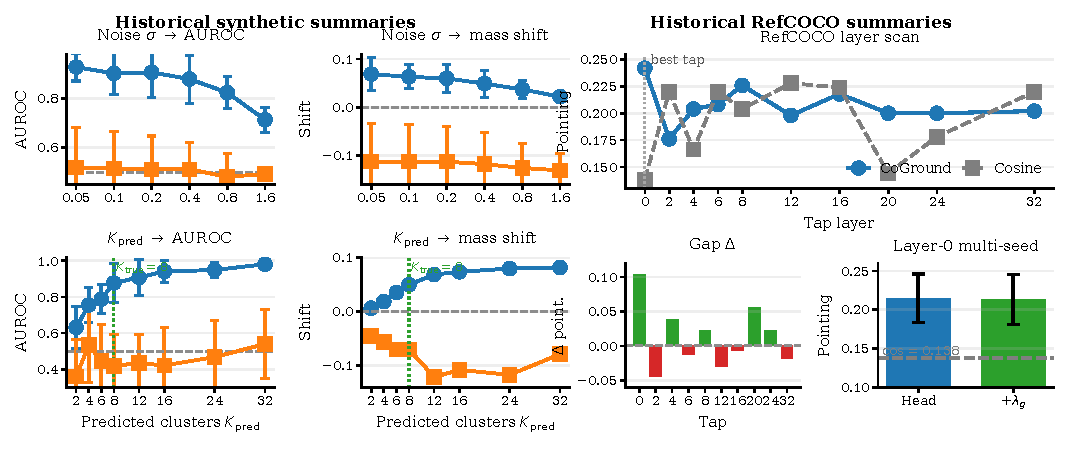
\includegraphics[width=\textwidth]{results_summary.pdf}
\caption{Historical exploratory summaries; bars denote the original reported standard deviations. Left: on synthetic data, \method\ outperforms the unconstrained low-rank baseline across the full noise sweep and remains robust when $K_{\mathrm{pred}}$ is misspecified around $K_{\mathrm{true}}=8$. Right: on frozen Gemma 4 E2B + RefCOCO, the gain over cosine is concentrated at the earliest tap, and the layer-zero panel retains the head and grounding-combo observations. The invalid decoding-combo row is excluded; no corrected experiment is shown. Exact values appear in Tables~\ref{tab:synthetic_massive}--\ref{tab:lt0_multiseed}.}
\label{fig:results_summary}
\end{figure}

The historical summaries are consistent with H1 within the matched block generator. Across a $32\times$ noise range, CoGround stays well above chance while low-rank remains essentially chance-level on AUROC and consistently produces a \emph{negative} supported-mass shift. The paired AUROC tests range from $t=9.32$ to $20.16$, and the paired supported-mass-shift tests range from $t=8.81$ to $17.34$; all corresponding $p$-values are below $10^{-7}$. These reported statistics cannot be independently recomputed without the per-run outputs, and the matched block generator alone cannot establish broad superiority of simplex constraints. NMF remains strong on this stylized generator, so the comparison concerns the simplex-constrained learned factorization relative to the unconstrained low-rank control.

\subsection{Robustness to cluster-count mismatch}

The historical cluster-count study considers the setting in which the true latent cluster count is unknown. The lower-left and lower-right synthetic panels in Figure~\ref{fig:results_summary} (exact values in Table~\ref{tab:kmismatch}) fix $K_{\mathrm{true}}=8$ and vary the predicted cluster count from $2$ to $32$ at $\sigma=0.2$, aggregating over 10 seeds per setting.

The reported means support the descriptive H2 trend within this generator family. CoGround degrades gracefully when $K_{\mathrm{pred}}$ is too small and improves monotonically in mean performance as $K_{\mathrm{pred}}$ becomes larger than $K_{\mathrm{true}}$, reaching AUROC $0.981$ at $K_{\mathrm{pred}}=32$. The low-rank control, by contrast, remains near chance across the whole sweep and keeps a negative supported-mass shift at every tested $K$. Within this generator family, over-parameterization therefore acts as a refinement of the support score rather than as a source of collapse.

\subsection{RefCOCO layer sensitivity and multi-seed observations}

The real-data results provide a second diagnostic perspective. The first question is whether a trained head beats a same-layer cosine baseline uniformly across the LM stack. The right block of Figure~\ref{fig:results_summary} answers that question with a 10-tap single-seed scan and a layer-$0$ multi-seed summary; exact values remain in Tables~\ref{tab:layertap_scan} and \ref{tab:lt0_multiseed}.

The layer scan sharpens the interpretation of the layer sensitivity result. The gain over same-layer cosine is \emph{not} uniform across taps: it is clearly strongest at layer $0$, where the head improves pointing by $+0.104$, and mostly disappears or changes sign at deeper taps. The cosine baseline itself is non-monotone, peaking around layers $12$--$16$, which suggests that raw similarity and learned co-clustering exploit different parts of the stack. The safest interpretation is therefore that the learned head adds the most value before the LM has strongly contextualized the visual tokens.

The layer-$0$ multi-seed panel in Figure~\ref{fig:results_summary} then tests that best tap directly across five seeds and adds two combo ablations; Table~\ref{tab:lt0_multiseed} retains the full Pointing / Recall@5 / AUROC breakdown. The main comparison is head-only CoGround versus the deterministic cosine baseline at the same tap.

The reported five-seed head pointing is $0.215\pm0.031$ against $0.138$ for cosine; the original test reports $t=5.60$, $p=0.005$. The available aggregate uses population standard deviation for these pointing values; sample standard deviation is about $0.0343$. A trained head versus untrained cosine cannot attribute the difference to co-clustering. Pointing asks whether the maximum-scoring patch is inside a box, whereas the reported AUROC $0.495\pm0.008$ is near chance and does not establish global spatial ranking. Hidden state zero is the embedding-level representation before transformer contextualization. The observation is therefore an early-feature probe, not evidence of recovered grounding in deep decoder layers.

The historical grounding combo reports $t=-0.30$, $p=0.78$ against the head. The decoding-combo condition did not enable a decoding module, so its identical values are not a no-harm ablation and are omitted from the result table and figure. No hallucination-reduction conclusion follows.

\subsection{Hypothesis status}

H1 and H2 have historical support only within a matched block-generator regime; overlapping and continuous structures need new measurements. H3 is an exploratory early-layer observation confounded by learned capacity and a custom split. H4 is not established: the decoding condition was inactive, and grounding compatibility needs a controlled comparison. No end-to-end generation or transfer improvement is claimed.

\subsection{Corrected prospective protocol}
The released code compares CoGround with a direct bilinear predictor and an MLP predictor that reuses the same bilinear projection and two head architectures without simplex assignments or $B$. Its trainable parameter count exactly matches CoGround when ranks and hidden dimensions agree. All methods must use the same official REFER splits, referring phrases, layer taps, seeds, update budget, and true grounding targets. Fixed-affinity, occupancy-solver, identity-$B$, sigmoid-membership, shuffled-target, and independent-decoding-state controls test separate mechanisms.

Grounding targets and metrics now share a row-major patch-center convention. Verified rectangular grids can be configured; unknown layouts, crops, tiles, and packed tokens require a model-specific mapping. Original image aspect ratio does not identify processor geometry. Token phrases are aligned in the actual multimodal sequence. A box with no positive patch center counts as a pointing/recall miss; AUROC excludes one-class examples and reports its own denominator. Patch Recall@$k$ is a top-$k$ center hit, not detector proposal recall.

The planned two-A100 configuration uses bf16, per-device batch one, eight accumulation steps, and 3,000 optimizer updates. This is a nominal batch of 16; tail accumulation can be smaller. RefCOCOg dataset transfer and PaliGemma~2 backbone transfer are separate. Synthetic stress tests add overlapping and continuous structure. Generation must pair the same checkpoint with the prior enabled and disabled. The built-in caption scorer and adjacent baseline adapters are diagnostic proxies, not official reproductions. None of these corrected experiments was executed for this version.

\section{Limitations and Broader Impact}
\label{sec:limitations}

The historical summaries test one favorable synthetic generator and one earlier backbone setup on a custom split. Missing raw artifacts prevent full retrospective verification. The corrected source has unit-tested software contracts, not new benchmark measurements or a validated real-backbone/GPU integration. Block structure can be a poor bias for overlapping or continuous evidence. Pseudoinverse gradients can be unstable near rank changes, and stopping the reconstruction target does not alone prevent a trivial affinity. The generation prior is static and has a contextual-token versus vocabulary-embedding shift. Grounding metrics do not establish reduced hallucination, and the earlier inactive decoding condition provides no compatibility evidence.

The broader impact is also narrow. Better local grounding may reduce unsupported outputs in assistive, educational, or scientific interfaces, but it does not solve factuality in general. The same mechanism could also make surveillance, profiling, or intrusive OCR systems more reliable. I therefore present \method\ as a tool for local grounding and diagnosis, not as a general safety solution.

\section{Conclusion}
\label{sec:conclusion}

\method\ treats local alignment as a structured latent object. The algebra characterizes block reconstruction and a conditional supported-mass effect; the retained synthetic and RefCOCO summaries motivate further tests but do not establish an advantage attributable to co-clustering. Corrected learned controls, structural stress tests, and an actual vocabulary-logit intervention make those questions testable. New matched experiments are required before drawing benchmark or generation conclusions.

\paragraph{Author and availability.}
Herv\'e Trinh, Independent Researcher.\\Correspondence: \href{mailto:trinh.herve@gmail.com}{\texttt{trinh.herve@gmail.com}}.\\Source and manuscript: \url{https://github.com/hervetrinh/coground-vlm}. Original repository material is CC BY 4.0; third-party assets retain their upstream terms.

\clearpage
\begingroup
\small
\setlength{\bibsep}{2pt}
\bibliographystyle{plainnat}
\bibliography{refs}
\endgroup

\clearpage
\appendix
\section{Proofs and Theoretical Clarifications}
\label{app:theory}

This appendix collects complete proofs for the formal properties stated in the main paper and adds one optimization result for the isolated co-clustering subproblem. The goal is to clarify what the mechanism guarantees, not to claim that the full VLM universally reduces hallucination.

\subsection{Optimal block reconstruction under fixed assignments}

\paragraph{Restated assumptions.}
For Proposition~\ref{prop:ls-block}, the matrices $U \in \R^{N_p \times K_p}$ and $V \in \R^{N_t \times K_t}$ are treated as fixed. Assume first that $U^\top U$ and $V^\top V$ are invertible; the pseudoinverse case is handled afterward.

\paragraph{Proof of Proposition~\ref{prop:ls-block}.}
Consider the objective
\[
f(B) = \|S-UBV^\top\|_F^2 = \mathrm{Tr}\big((S-UBV^\top)^\top(S-UBV^\top)\big).
\]
Expanding the trace gives
\[
f(B)=\mathrm{Tr}(S^\top S) - 2\,\mathrm{Tr}(S^\top U B V^\top) + \mathrm{Tr}(V B^\top U^\top U B V^\top).
\]
By cyclicity of the trace,
\[
\mathrm{Tr}(S^\top U B V^\top)=\mathrm{Tr}(B V^\top S^\top U)
\]
and
\[
\mathrm{Tr}(V B^\top U^\top U B V^\top)=\mathrm{Tr}(B^\top U^\top U B V^\top V).
\]
Differentiating with respect to $B$ yields
\[
\nabla_B f(B) = -2U^\top S V + 2U^\top U\,B\,V^\top V.
\]
Any minimizer therefore satisfies the normal equations
\[
U^\top U\,B\,V^\top V = U^\top S V.
\]
If $U^\top U$ and $V^\top V$ are invertible, the unique critical point is
\[
B^\star = (U^\top U)^{-1}U^\top S V (V^\top V)^{-1}.
\]
Because $f$ is a convex quadratic function of $B$, this critical point is the global minimizer. If one or both Gram matrices are singular, the same normal equations characterize the affine set of minimizers, and the Moore-Penrose pseudoinverse yields the minimum-norm solution
\[
B^\star = (U^\top U)^+ U^\top S V (V^\top V)^+.
\]
This proves Proposition~\ref{prop:ls-block}. \hfill $\square$

\subsection{Compression and exact recovery in the block-constant regime}

\paragraph{Restated assumptions.}
For Proposition~\ref{prop:rank-recovery}, $U$, $V$, and $B$ are arbitrary matrices for the rank statement. For the exact-recovery statement, $U$ and $V$ are hard-assignment matrices, so each row of $U$ and each row of $V$ contains a single $1$, and $S$ is assumed constant on every block induced by the corresponding row and column partitions.

\paragraph{Proof of Proposition~\ref{prop:rank-recovery}.}
The rank statement follows from the standard inequality
\[
\mathrm{rank}(ABC) \le \min\{\mathrm{rank}(A),\mathrm{rank}(B),\mathrm{rank}(C)\}.
\]
Applying it to $UBV^\top$ gives
\[
\mathrm{rank}(UBV^\top) \le \min\{\mathrm{rank}(U),\mathrm{rank}(B),\mathrm{rank}(V^\top)\}.
\]
Since $\mathrm{rank}(V^\top)=\mathrm{rank}(V)$, $\mathrm{rank}(U)\le K_p$, and $\mathrm{rank}(V)\le K_t$, the rank inequalities yield
\[
\mathrm{rank}(\hat S) \le \min\{\mathrm{rank}(U),\mathrm{rank}(B),\mathrm{rank}(V)\} \le \min\{K_p,K_t\}.
\]
For exact recovery, let $C_a$ be the set of patch indices assigned to block $a$ and $D_b$ the set of token indices assigned to block $b$. Because $U$ and $V$ are hard assignments, for every pair $(i,j)$ there is a unique pair $(a(i),b(j))$ such that $U_{i,a(i)}=1$ and $V_{j,b(j)}=1$. Hence
\[
(UBV^\top)_{ij} = \sum_{a=1}^{K_p}\sum_{b=1}^{K_t} U_{ia}B_{ab}V_{jb} = B_{a(i)b(j)}.
\]
If $S$ is block-constant, then there exist constants $\theta_{ab}$ such that $S_{ij}=\theta_{ab}$ whenever $(i,j)\in C_a\times D_b$. The occupancy-normalized estimator computes the average of $S$ over each block, so for every $(a,b)$,
\[
B_{ab} = \frac{1}{|C_a||D_b|}\sum_{i\in C_a}\sum_{j\in D_b} S_{ij} = \theta_{ab}.
\]
Therefore $(UBV^\top)_{ij}=\theta_{a(i)b(j)}=S_{ij}$ for every $(i,j)$, which proves exact reconstruction. \hfill $\square$

\subsection{Supported-mass monotonicity under the decoding bias}

\paragraph{Restated assumptions.}
For Proposition~\ref{prop:mass-shift}, fix a decoding step and define
\[
q_i(\lambda) = \frac{\exp(a_i + \lambda c_i)}{\sum_{\ell=1}^{N_p}\exp(a_\ell + \lambda c_\ell)}.
\]
Let $G\subseteq\{1,\dots,N_p\}$ be the supported set. The required assumption is the ordering condition $c_i\ge c_j$ for all $i\in G$ and $j\notin G$.

\paragraph{Proof of Proposition~\ref{prop:mass-shift}.}
Define
\[
Q_G(\lambda) = \sum_{i\in G} q_i(\lambda), \qquad Z(\lambda) = \sum_{\ell=1}^{N_p}\exp(a_\ell + \lambda c_\ell).
\]
The derivative of the softmax probabilities is
\[
\frac{dq_i}{d\lambda} = q_i(\lambda)\left(c_i - \sum_{\ell=1}^{N_p} q_\ell(\lambda)c_\ell\right).
\]
Summing over $i\in G$ gives
\[
\frac{dQ_G}{d\lambda} = \sum_{i\in G} q_i\big(c_i-\mathbb{E}_{q(\lambda)}[c]\big).
\]
Now define the conditional means
\[
\mu_G = \frac{1}{Q_G}\sum_{i\in G} q_i c_i, \qquad \mu_{\bar G} = \frac{1}{1-Q_G}\sum_{j\notin G} q_j c_j.
\]
Then
\[
\mathbb{E}_{q(\lambda)}[c] = Q_G\mu_G + (1-Q_G)\mu_{\bar G},
\]
so
\[
\frac{dQ_G}{d\lambda} = Q_G\big(\mu_G - \mathbb{E}_{q(\lambda)}[c]\big) = Q_G(1-Q_G)(\mu_G-\mu_{\bar G}).
\]
Under the ordering assumption, every score inside $G$ is at least as large as every score outside $G$, which implies $\mu_G\ge \mu_{\bar G}$. Therefore
\[
\frac{dQ_G}{d\lambda} \ge 0.
\]
If the inequality is strict on a subset carrying nonzero probability mass and if $0<Q_G<1$, then $\mu_G>\mu_{\bar G}$ and the derivative is strictly positive. This proves Proposition~\ref{prop:mass-shift}. \hfill $\square$

\subsection{Monotone descent for the isolated co-clustering subproblem}

\begin{theorem}
\label{thm:alt-descent}
Consider the regularized objective
\[
\mathcal{J}(U,V,B) = \|S-UBV^\top\|_F^2 + \lambda_U R_U(U) + \lambda_V R_V(V) + \lambda_B\|B\|_F^2,
\]
where $U$ and $V$ lie in products of simplices, $R_U$ and $R_V$ are continuous and bounded below, and $\lambda_B>0$. Suppose that each iteration performs: (i) an exact minimization over $B$ with $(U,V)$ fixed; (ii) a descent-guaranteed update of $U$ with $(V,B)$ fixed; and (iii) a descent-guaranteed update of $V$ with $(U,B)$ fixed. Then the sequence $\mathcal{J}(U^t,V^t,B^t)$ is monotone nonincreasing and converges to a finite value. No stationarity or convergence claim is made for the stochastic neural trainer used in the experiments.
\end{theorem}

\paragraph{Proof.}
By exact minimization over $B$,
\[
\mathcal{J}(U^t,V^t,B^{t+1}) \le \mathcal{J}(U^t,V^t,B^t).
\]
By the descent property of the $U$ update,
\[
\mathcal{J}(U^{t+1},V^t,B^{t+1}) \le \mathcal{J}(U^t,V^t,B^{t+1}).
\]
By the descent property of the $V$ update,
\[
\mathcal{J}(U^{t+1},V^{t+1},B^{t+1}) \le \mathcal{J}(U^{t+1},V^t,B^{t+1}).
\]
Chaining the three inequalities yields
\[
\mathcal{J}(U^{t+1},V^{t+1},B^{t+1}) \le \mathcal{J}(U^t,V^t,B^t),
\]
so the objective sequence is monotone nonincreasing. Every term in $\mathcal{J}$ is bounded below: the reconstruction term and ridge term are nonnegative, while the regularizers are bounded below by assumption. Hence $\mathcal{J}(U^t,V^t,B^t)$ converges to a finite limit.

This proves objective-value convergence for the specified isolated descent scheme only. It does not prove convergence of the joint neural training procedure or stationarity without stronger optimization assumptions. \hfill $\square$

\section{Additional Numerical Tables}
\label{app:numerics}

This appendix preserves the historical numeric summaries underlying the synthetic and RefCOCO panel groups in Figure~\ref{fig:results_summary}.

\begin{table}[htbp]
\caption{Massive synthetic comparison with an unconstrained low-rank factorization. Means and standard deviations are over 20 seeds; paired two-sided $t$-statistics compare CoGround against low-rank on AUROC and supported-mass shift.}
\label{tab:synthetic_massive}
\centering
\footnotesize
\setlength{\tabcolsep}{3pt}
\resizebox{\linewidth}{!}{%
\begin{tabular}{@{}ccccccc@{}}
\toprule
$\sigma$ & CoGround AUROC & Low-rank AUROC & $\Delta$AUROC & CoGround shift & Low-rank shift & $t_{\mathrm{A}} / t_{\mathrm{S}}$ \\
\midrule
0.05 & $0.928\pm0.057$ & $0.518\pm0.163$ & $+0.410$ & $+0.069\pm0.035$ & $-0.113\pm0.079$ & $13.58 / 8.81$ \\
0.10 & $0.902\pm0.087$ & $0.514\pm0.152$ & $+0.388$ & $+0.063\pm0.025$ & $-0.113\pm0.077$ & $10.27 / 9.27$ \\
0.20 & $0.906\pm0.101$ & $0.511\pm0.136$ & $+0.395$ & $+0.060\pm0.029$ & $-0.113\pm0.073$ & $9.32 / 9.26$ \\
0.40 & $0.879\pm0.098$ & $0.511\pm0.108$ & $+0.368$ & $+0.049\pm0.028$ & $-0.118\pm0.065$ & $11.19 / 10.12$ \\
0.80 & $0.824\pm0.064$ & $0.481\pm0.094$ & $+0.343$ & $+0.037\pm0.018$ & $-0.126\pm0.051$ & $14.27 / 12.66$ \\
1.60 & $0.713\pm0.050$ & $0.492\pm0.025$ & $+0.222$ & $+0.022\pm0.010$ & $-0.131\pm0.035$ & $20.16 / 17.34$ \\
\bottomrule
\end{tabular}%
}
\end{table}

\begin{table}[htbp]
\caption{Robustness to cluster-count misspecification at $\sigma=0.2$ with $K_{\mathrm{true}}=8$. Means and standard deviations are over 10 seeds.}
\label{tab:kmismatch}
\centering
\footnotesize
\setlength{\tabcolsep}{3pt}
\resizebox{\linewidth}{!}{%
\begin{tabular}{@{}cccccc@{}}
\toprule
$K_{\mathrm{pred}}$ & CoGround AUROC & Low-rank AUROC & $\Delta$AUROC & CoGround shift & Low-rank shift \\
\midrule
2 & $0.631\pm0.114$ & $0.359\pm0.206$ & $+0.272$ & $+0.006$ & $-0.045$ \\
4 & $0.755\pm0.096$ & $0.533\pm0.209$ & $+0.222$ & $+0.018$ & $-0.057$ \\
6 & $0.788\pm0.080$ & $0.446\pm0.202$ & $+0.342$ & $+0.035$ & $-0.070$ \\
8 & $0.877\pm0.107$ & $0.419\pm0.173$ & $+0.458$ & $+0.049$ & $-0.070$ \\
12 & $0.908\pm0.099$ & $0.433\pm0.157$ & $+0.475$ & $+0.068$ & $-0.121$ \\
16 & $0.941\pm0.061$ & $0.421\pm0.209$ & $+0.520$ & $+0.073$ & $-0.108$ \\
24 & $0.949\pm0.043$ & $0.467\pm0.201$ & $+0.483$ & $+0.079$ & $-0.117$ \\
32 & $0.981\pm0.025$ & $0.540\pm0.192$ & $+0.441$ & $+0.081$ & $-0.079$ \\
\bottomrule
\end{tabular}%
}
\end{table}

\begin{table}[htbp]
\caption{Single-seed RefCOCO layer scan (seed 17). The trained head is compared against a same-layer cosine affinity baseline with no learned head.}
\label{tab:layertap_scan}
\centering
\footnotesize
\setlength{\tabcolsep}{3pt}
\begin{tabular}{@{}cccc@{}}
\toprule
Tap & Head pointing & Cosine pointing & $\Delta$ \\
\midrule
0 & \textbf{0.242} & 0.138 & $+0.104$ \\
2 & 0.176 & 0.220 & $-0.044$ \\
4 & 0.204 & 0.166 & $+0.038$ \\
6 & 0.208 & 0.220 & $-0.012$ \\
8 & 0.226 & 0.204 & $+0.022$ \\
12 & 0.198 & 0.228 & $-0.030$ \\
16 & 0.218 & 0.224 & $-0.006$ \\
20 & 0.200 & 0.144 & $+0.056$ \\
24 & 0.200 & 0.178 & $+0.022$ \\
32 & 0.202 & 0.220 & $-0.018$ \\
\bottomrule
\end{tabular}
\end{table}

\begin{table}[htbp]
\caption{Five-seed RefCOCO evaluation at layer $0$. The original reported means and population standard deviations are over seeds $17$--$21$; these are historical observations.}
\label{tab:lt0_multiseed}
\centering
\footnotesize
\setlength{\tabcolsep}{3pt}
\resizebox{\linewidth}{!}{%
\begin{tabular}{@{}lcccc@{}}
\toprule
Condition & Pointing & Recall@5 & AUROC & Statistical note \\
\midrule
Cosine baseline & $0.138$ & $0.530$ & $0.500$ & Reference \\
Head only & $0.215\pm0.031$ & $0.559\pm0.039$ & $0.495\pm0.008$ & vs cosine: $t=5.60$, $p=0.005$ \\
+$\lambda_g=0.5$ & $0.213\pm0.032$ & $0.551\pm0.049$ & $0.505\pm0.003$ & vs head: $t=-0.30$, $p=0.78$ \\
\bottomrule
\end{tabular}%
}
\end{table}


\end{document}
